\section{Defending against Malware Attacks}
\label{sec:mitigating_sca}

In this section, we show that \framework offers a novel approach to mitigate the
risk of leaking sensitive user data.

\subsection{Testing \framework{} against Real-world Malicious Apps}
\label{sec:malicious_apps}

To assess \framework{}'s defense against real-world malicious apps, we selected 30 of the most downloaded apps recently banned from the Google Play Store. Since these apps were no longer available there, we obtained their latest versions from third-party platforms. We then analyzed their malicious behavior using sensitive API access logs recorded by \framework{}.

Table \ref{tab:malicious_apps} summarizes the malicious behaviors identified in the 30 analyzed apps. We anticipate that users can detect similar threats using \framework{}. In the future, we aim to enhance \framework{} to proactively notify users of suspected malicious activities.

\noindent Malicious behaviors fell under 4 major categories:

\mysubheading{Upload sensitive data to the internet.} Some apps transmitted large amount of data in the background. For instance, \textit{PhoneFinder by Clapping} likely uploaded user audio data, as it had microphone access. Since revoking or spoofing this permission would break its functionality, \framework{} restricted its internet access to protect user privacy.

\mysubheading{Accessing sensitive data unnecessarily.} Many malicious apps accessed irrelevant sensitive data. \textit{Amazing Video Editor} and \textit{Keyboard Themes} accessed contacts, while \textit{Instant Speech Translation} accessed photos. Denying these permissions caused app crashes, but \framework{} successfully spoofed the data without affecting functionality.

\mysubheading{Accessing data without user knowledge.} Some apps accessed sensitive data unexpectedly. \textit{Free Translator Photo} attempted to access images without a translation request. \textit{Bus Driver Simulator} used accelerometer and gyroscope data while running in the background. \framework{} effectively spoofed sensitive data, allowing users to configure policies to restrict access only when the app is in the background. \textit{GeoSpot: GPS Tracker} tracked user locations even when not requested. \framework{} spoofed the location but required manual user intervention to differentiate between legitimate and unauthorized background tracking.

\mysubheading{Sending SMS messages.} Apps like \textit{Private SMS} used \texttt{SMSManager.sendTex- tMessage()} without user consent. Such apps have been linked to financial fraud via premium SMS subscriptions. \framework{} blocked these messages, though this also affected app functionality. This highlights a limitation where spoofing cannot prevent malicious behavior if the app genuinely requires the data for its core features.

\begin{table}
    {\centering
    % \begin{tabular}{>{\arraybackslash} m{4.1cm}  >{\centering\arraybackslash} m{2cm} >{\centering\arraybackslash} m{5.15cm} >{\centering\arraybackslash} m{5.15cm}}
    \begin{tabular}{p{\linewidth}} 
         \toprule
         \textbf{Malicious behavior:} Upload sensitive data to internet\\
         \textbf{Apps (downloads):}
         All Good PDF Scanner (10M+), Fast PDF Scanner (5M+), PhoneFinder by
         Clapping (5M+), What's Me Sticker (1M+)\\
         \textbf{\framework:} Limit internet access to the app\\
         \midrule
         \midrule
         \textbf{Malicious behavior:} Access sensitive user data like Contacts, Location, Audio,
         and Sensors unnecessarily\\
         \textbf{Apps (downloads):} Amazing Video Editor (5M+), CapCut Pro (5M+), Instant Speech Translation (5M+), Keyboard Themes (5M+),
         Launcher iOS 15 (5M+) \\
         \textbf{\framework:} Deceived all the unnecessary user data requested without crashing the apps\\
         \midrule
         \midrule
         \textbf{Malicious behavior:} Accessing data without user knowledge\\
         \textit{Accessing sensor data in the background}\\
         \textbf{Apps (downloads):} Bus Driver Simulator (5M+), Bus - Metrolis 2021 (1M+),
         Fingerprint Changer (1M+), Fingerprint Defender (1M+), Lifeel - scan and test (5M+),
         Locker Tool (5M+), OFFRoaders - Survive (5M+), Racers Car Driver (5M+), Safe Lock (5M+),
         Slime Simulator (5M+), Smart Spot Locator (1M+), Unique Keyboard (5M+) \\
         \textbf{\framework:} Allowed the apps to access the sensor
         data in the foreground but not in the background\\
         \midrule
         
         \textit{Camera access without user consent and knowledge}\\
         \textbf{Apps (downloads):} Free Translator Photo (5M+), Handy Translator Pro (10M+),
         Heart Rate and Pulse Tracker (5M+), Heart Rhythm (1M+),
         My Chat Translator (5M+) \\
         \textbf{\framework:} Deceived camera data fed into the app\\
         \midrule
         
         \textit{Location continuously tracked by app}\\
         \textbf{Apps (downloads):} Geospot: GPS Tracker (5M+), iCare - Find Location (5M+) \\
         \textbf{\framework:} Deceived location data according to user policy\\
         \midrule
        \midrule
        \textbf{Malicious behavior:} Detected accessing Send SMS API without user knowledge\\
        \textbf{Apps (downloads):} Private SMS (5M+), Mint Left Messages (1M+) \\
        \textbf{\framework:} Blocked access to send SMS but not from reading SMS as per user policy\\
        \bottomrule
    \end{tabular}
    }
    \caption{Malicious behavior of Android apps banned by Google and the actions taken by \framework 
    to protect user privacy.}
    \label{tab:malicious_apps}
\end{table}

% \begin{table*}
%     {\centering
%     \begin{tabular}{>{\centering\arraybackslash} m{4.1cm}  >{\centering\arraybackslash} m{2cm} >{\centering\arraybackslash} m{5.15cm} >{\centering\arraybackslash} m{5.15cm}}
%         \hline
%          \textbf{Malicious App} & \textbf{\#Downloads (in millions)} & \textbf{Malicious activities detected by \framework{}} & \textbf{Actions performed by \framework{}} \\
%          \hline
         
%          All Good PDF Scanner & 10+ & Cam, Net & SUP(Cam), SB\\
%          Fast PDF Scanner & 5+ & Cam, Net & SUP(Cam), SB \\
%          PhoneFinder by Clapping & 5+ & Net, Aud & SUP(Aud), UDP(Net), SB \\
%          What's Me Sticker & 1+ & Cam, Net & SUP(Cam), UDP(Net), SB \\
%          \hline         
         
%          Amazing Video Editor & 5+ & Acc, Aud, Cam, Con, Loc, Net & SUP(Aud, Cam), UDP(Acc, Con, Loc), SB\\
%          CapCut Pro & 5+ & Aud, Cam, Con, Loc, Net & SUP(Aud, Cam), UDP(Con, Loc), SB\\
%          \hline
         
%          Bus Driver Simulator & 5+ & Net & UDP(Net), SB \\
%          Bus - Metrolis 2021 & 1+ & Net & UDP(Net), SB \\
%          Fingerprint Changer & 1+ & Net & SB \\
%          Fingerprint Defender & 1+ & Net & SB \\
%          Lifeel - scan and test & 5+ & Net & SB \\
%          Locker Tool & 5+ & Net & UDP(Net), SB \\
%          OFFRoaders - Survive & 5+ & Net & UDP(Net), SB \\
%          Racers Car Driver & 5+ & Net & UDP(Net), SB \\
%          Safe Lock & 5+ & Net & UDP(Net), SB \\
%          Slime Simulator & 5+ & Net & UDP(Net), SB \\
%          Smart Spot Locator & 1+ & Net & SB\\
%          Unique Keyboard & 5+ & Net & UDP(Net), SB \\
%          \hline

%          Private SMS & 5+ & Acc, Cam, CLg, Con, Msg, Net & SUP(Acc, Cam, CLg, Con, Msg), SB\\
%          Mint Left Messages & 1+ & Aud, Cam, CLg, Con, Msg, Net & SUP(Aud, CLg, Cam, Con, Msg), SB\\
%          \hline
         
%          Free Translator Photo & 5+ & Cam & SUP(Cam), SB \\
%          Handy Translator Pro & 10+ & Acc, Cam & UDP(Acc), SUP(Cam), SB \\
%          My Chat Translator & 5+ & Acc, Cam & UDP(Acc), UDU(Cam), SB \\
%          \hline
         
%          Geospot: GPS Tracker & 5+ &  Loc, Net  & SUP(Loc), SB \\
%          iCare - Find Location & 5+ &  Cam, Loc, Net  & SUP(Loc), UDP(Cam), SB\\
%          \hline
         
%          Heart Rate and Pulse Tracker & 5+ & Cam & UDP(Cam), SB \\         
%          Heart Rhythm & 1+ & Cam & UDP(Cam), SB \\
%          \hline
         
%          Instant Speech Translation & 5+ & Acc, Aud, Cam & UDP(Acc, Cam), SUP(Aud), SB \\
%          \hline
         
%          Keyboard Themes & 5+ & Acc, Con & UDP(Acc, Con), SB \\
%          Launcher iOS 15 & 5+ & Acc, Aud, Cam, Con, Loc, Net & UDU(Acc, Aud, Cam, Con, Loc, Net), SB \\
%          \hline
         
         
         
         
         
         

%          \hline
%          \multicolumn{4}{l}{\footnotesize \textbf{Acc}: Account, \textbf{Aud}: Audio, \textbf{Cam}: Camera, \textbf{CLg}: Call Logs, \textbf{Con}: Contacts, \textbf{Loc}: Location, \textbf{Msg}: SMS, \textbf{Net}: Network } \\
         
%          \hline
%          \multicolumn{4}{p{16.4cm}}{\footnotesize \textbf{SB}: Sandboxing apps and isolating from external world and other apps installed on the device to protect user privacy and mitigate attacks, \textbf{SUP}: Selective user data protection to ensure app functionality without compromising user data, \textbf{UDP}: Deceiving unnecessary dangerous permissions requested to ensure user privacy without crashing app, \textbf{UDU}: Detecting and blocking unexpected user data usage } \\
%          \hline
%     \end{tabular}
%     }
%     \caption{Malicious Android Apps banned by Google.}
%     \label{tab:malicious_apps}
% \end{table*}


\subsection{Mitigating Side-Channel Attacks}
\label{sec:side_channel_attack}
Side-channel attacks exploit unintended information leaks, such as sensor readings, power consumption, or electromagnetic signals, to infer sensitive data. Mobile devices, with their numerous sensors and communication interfaces, are particularly vulnerable to such attacks, which can compromise passwords, cryptographic keys, or biometric data.

Recent research~\cite{hasan2013sensing, simon2013pin, ba2020learning, shen2015input} has highlighted the risks posed by so-called \textit{Normal} Permissions—those that allow access to seemingly harmless data like accelerometer and gyroscope readings without requiring explicit user approval. However, attackers have leveraged these permissions to extract sensitive user information.

To address this privacy threat, \framework{} provides an innovative defense against side-channel attacks by selectively modifying the permissions granted to apps. By deceiving user data, \framework{} disrupts the ability of malicious apps to collect meaningful information through side channels.

To demonstrate \framework{}'s effectiveness, we tested it against \textit{GyroSec}~\cite{lin2019motion}, an Android app that covertly records accelerometer and gyroscope data. \textit{GyroSec} then transmits this data to a remote server, where machine-learning algorithms predict touch inputs on the screen—posing a serious privacy risk. Our experiments confirmed that \textit{GyroSec} could execute this side-channel attack without any restrictions from the Android Permission Framework.

By configuring \framework{} to deceive \textit{GyroSec}, we successfully logged every instance of data access and notified users of unauthorized background resource usage. Using the \textit{Policy Configurator}, we manipulated the accelerometer and gyroscope sensor readings to return constant values, effectively neutralizing the attack. Figure \ref{fig:tchPredict} illustrates the drastic reduction in \textit{GyroSec}'s prediction accuracy. The accuracy dropped from \textbf{81.22\%} to \textbf{5.36\%}, demonstrating \framework{}'s effectiveness in mitigating permission-based side-channel attacks.

\begin{figure}[t]
\centering
\begin{subfigure}{0.35\linewidth}
    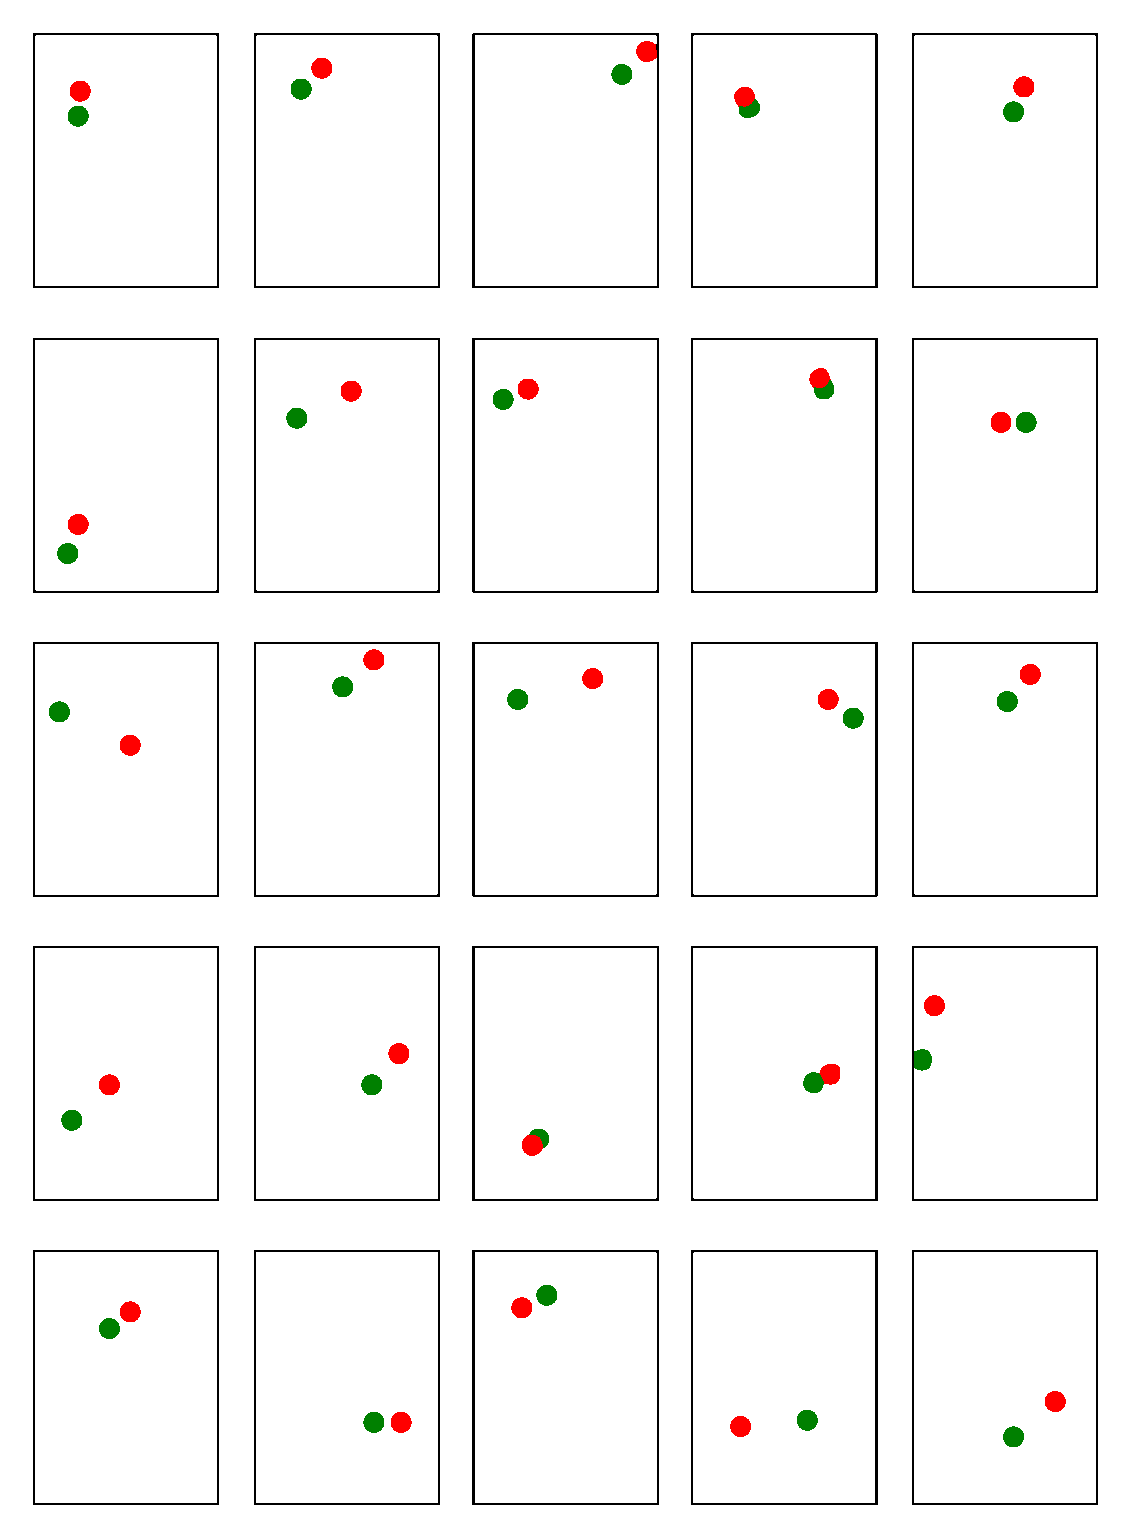
\includegraphics[width=\linewidth]{Figures/Side Channel Attacks/touch_prediction_samples_by_GyroSec_without_Deceiver.pdf}
    \caption{Without \framework{}}
    % \caption{Without \framework{} (High Accuracy achieved using true sensor readings)}
    \label{fig:tchPredict_wo_frmwrk}
\end{subfigure}
\hspace{0.9mm}
\begin{subfigure}{0.35\linewidth}
    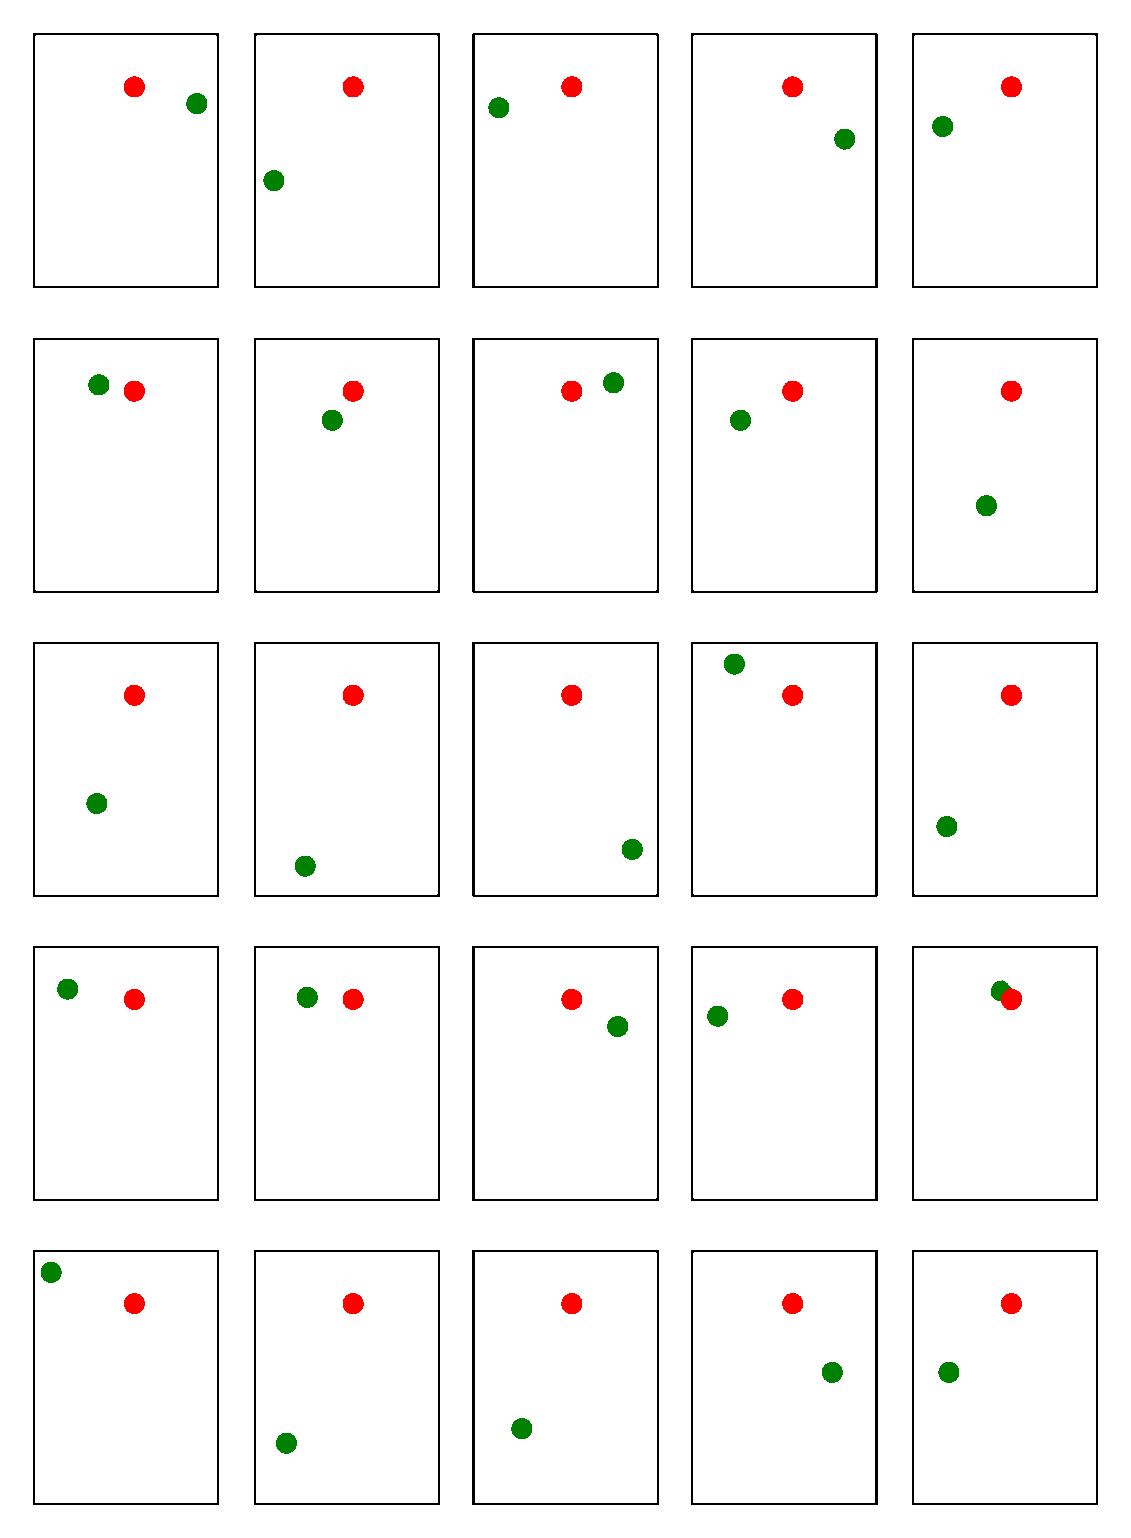
\includegraphics[width=\linewidth]{Figures/Side Channel Attacks/touch_prediction_samples_by_GyroSec_with_Deceiver.pdf}
    \caption{With \framework{}}
    \label{fig:tchPredict_w_frmwrk}
\end{subfigure}
\caption{Touch predicitions made by \textit{Gyrosec} server based on sensor readings received.}
\label{fig:tchPredict}
\end{figure}

\textit{Overall, this section shows that \framework could effectively stop most 
malicious behaviors giving better control to users over their sensitive data.}
